%************************************************
\chapter{The Client Tier}
\label{ch:client-tier}
%************************************************

\section{Introduction}

The client tier is very close to the user. Typically, it consists of components executed on a device that provides some sort of user interface. The user interface might be a \ac{GUI} or a \ac{CLI}. There are many different ways to design the client tier, which are reviewed in this chapter.

\section{Thin web clients}

\marginpar{If it is really, really thin, the client does not execute any logic. Views generated by the server are simply rendered by the browser. Every user action triggers an HTTP request and a full page reload.}

A very common situation is when users interact with the application via a web browser. They launch the browser, type in a URL and get to a user interface that has been generated by the server-side components of the application. The term \emph{thin} means that there is very little logic, and therefore code, running on the server side. Some applications are really, really thin: the browser receives HTML, stylesheets and media files and simply renders them. The application does not use any client-side Javascript, so there is no code executed in the browser. But many applications add a bit of meat around that structure. Some Javascript code is added and executed in the browser, for instance to validate data entered in forms.

\section{Rich web client clients}

\marginpar{Rich indicates that there is more interactivity in the user interface, which mandates for some of the UI logic to be running on the client. The logic is implemented in Javascript functions, executed by the engine embedded in the browser.}

When the amount of Javascript code grows, the web clients become \emph{richer}. Think about social network applications, online games, or complex business applications: a lot of them now have a very interactive user interface, which requires code to be executed in the browser. The term \ac{SPA} refers to a pattern that has become very popular, and that is enabled by Javascript frameworks such as Angular, React or Vue. Here, most of the user interaction is handled on the client side, including page navigation. At the beginning of the session, the user visits a URL and fetches a skeleton that bootstraps the application. He sees the entry page in the application and start interacting with it. As he clicks on links and buttons, the entire page is never reloaded in the browser. Instead, the browser fetches HTML fragments and application data. It injects these elements in the page skeleton and sometimes gives the impression that a page has been reloaded. Be aware that even if the URL changes in the navigation bar, it is possible that a full page has not been requested by the client.

\section{Native GUI clients}

\marginpar{In the past, many things were not possible in a web browser. This is the reason why some applications provided a rich desktop client. Today, browsers provide a rich environment and a viable alternative most of the time. Mobile devices are still an area where native clients have benefits.}

On the desktop, there used to be a time where many business applications did not use a browser on the client side. Instead, they used a rich client developed with a GUI toolkit such as Swing. One reason for doing that was the need for a high degree of interactivity, at a time where browser capabilities where lacking (we are talking about the early 2000s). Today, there are still some scenarios where a rich desktop client makes sense, but they are not the majority.

However, there is another reason why a lot of multi-tiered systems include a native client: the support for mobile users. In this case, many developers make the choice to implement a native application, for instance on iOS or Android.

When the application includes a native client, one question that needs to be answered is how the client-side components communicate with the server-side components. Today, the most common protocol used for that purpose is HTTP. In this case, HTTP is used to transport data (e.g. JSON, XML) and not HTML documents. In the past, many companies used to build rich clients in Java and use the \ac{RMI} protocol to to handle communications between objects on the client and the server side. This is not a scenario that we will look in details in this book.

\section{CLI clients}

\marginpar{When you type a command in a terminal, you might well be interacting with the client component of a multi-tiered application}

Many applications provide a text-based interface, sometimes in addition to a graphical user interface. One of the benefits of such an interface is that it facilitates scripting and automation. When using a \ac{CLI}, one might sometimes have the impression that everything runs locally. This is not correct: many programs that implement a \ac{CLI} are network clients and make remote calls to a service. In other words, when the user types a command on the terminal, the program might send an HTTP request to a remote service, process its reply and format a message on the terminal.

Many applications are designed with the idea that a user will drive the interaction and trigger the execution of business logic. But there are also a lot of applications where the entity initiating the work is a software agent. Think about automation scripts executed periodically. Think about IoT sensors and actuators that send data to a cloud application.

\section{Communication protocols}

The previous paragraphs have already mentioned some of the communication protocols used between the client tier and the server tiers. These protocols are shown in Figure \ref{fig:client-tier}. Here are few comments about every scenario:

\begin{itemize}
\item For thin clients, HTTP is used to transport HTML documents (and other web assets like stylesheets and images). Since there is no logic executed on the client, there is no point to send structured business data from the server to the client.
\item For rich web clients, HTTP is used to transport UI assets (HTML, stylesheets, media files) but also business data. This data is requested by scripts running in the browser, formatted and injected in the page UI. The figure mentions JSON as a format for serializing business data, but there are other formats (XML, CSV, binary formats, etc.).
\item For native clients, HTTP is also often used as the underlying transport protocol. But in this case, there is no web page, so what is transported is structured business data.
\item Finally, the case of legacy Java clients is a bit particular. In this case, the objects created in the \ac{JVM} on the client may use the \ac{RMI} protocol over \ac{IIOP} to make method calls to objects created in the \ac{JVM} on the server side. In this case, the figure suggests that the call can be done directly to the business tier.
\end{itemize}

\begin{figure}[]
	\centering
    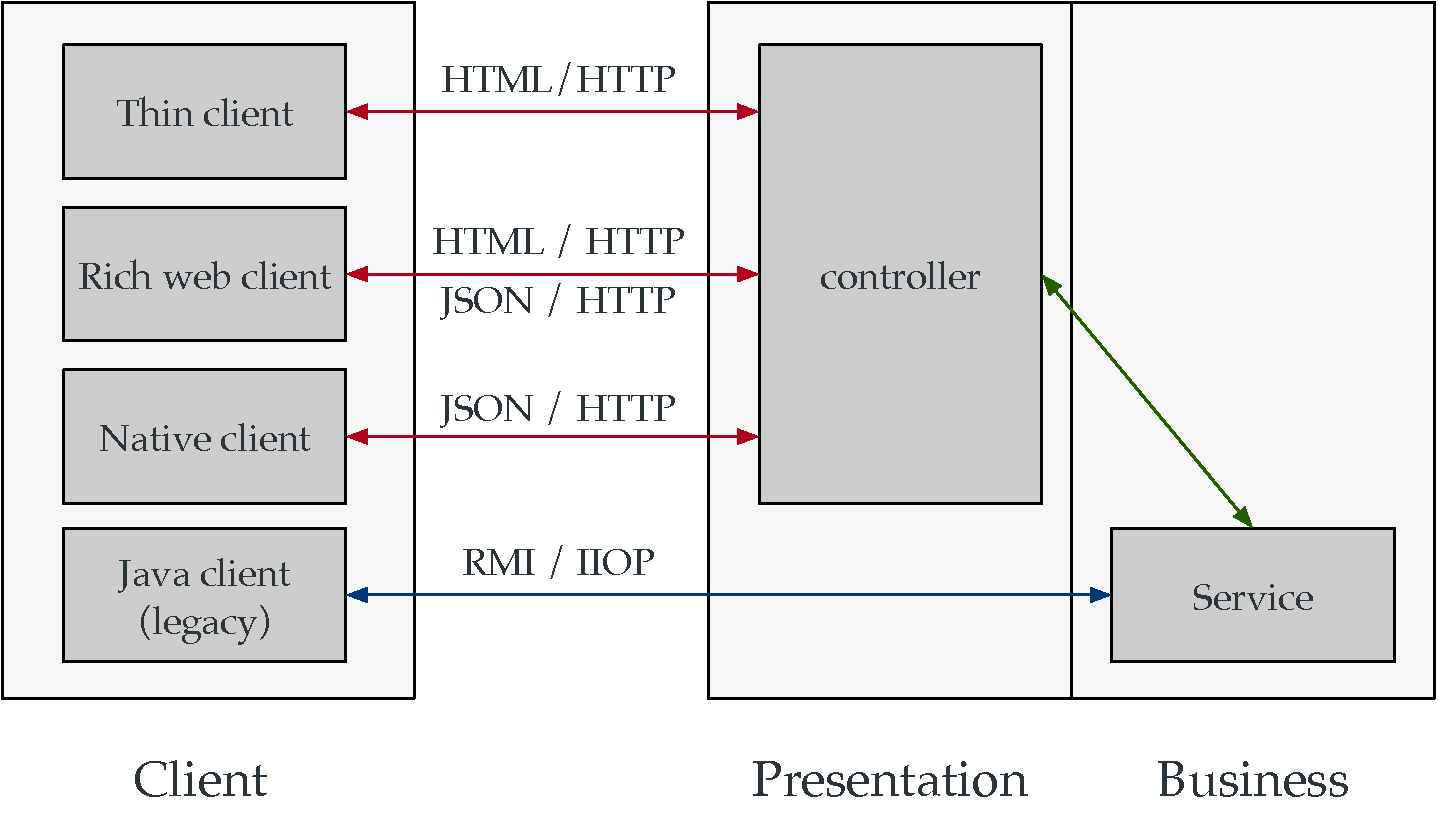
\includegraphics[width=1.0\linewidth]{Figures/client-tier.pdf}
	\caption{Interactions between the client and server tiers}
  \label{fig:client-tier}
\end{figure}

\section{Questions}

To answer these questions, you will need to have read the chapter but also to have done some research. Make sure that you are able to answer every question. Discuss your responses with your peers.

\begin{enumerate}
\item Let us consider Facebook. What kind of clients does the company use? Do not forget that a company always has external and internal applications.
\item What does the acronym AJAX mean and how does it relate to the client tier?
\item Give an example of a \ac{CLI} tool that you use and that is the client of a multi-tiered application.
\end{enumerate}

